\section{The Octave: Why Eight Ticks Are Forced}
\noindent\fbox{\parbox{0.97\linewidth}{%
\textbf{Section summary.}
This framework models the minimal stable closure in three dimensions as an \emph{eight-step} cycle (an ``octave'').
Two ingredients matter: (i) a counting statement (a 3-bit context space has eight states), and (ii) a dynamics statement (atomic updates move by one-bit steps),
which together motivate a Gray-adjacent 8-cycle as the canonical closure schedule.
These are conditional modeling statements: if the underlying closure is not three-bit or not atomic, the Octave premise would need revision.}}

\subsection{Minimal closure: why the period is eight in a three-bit context space}
We begin with a clean separation between \emph{what is assumed} and \emph{what follows}.

\paragraph{Assumption (context encoding).}
We assume the relevant ``closure state'' of a stable boundary is representable as three independent binary degrees of freedom (a 3-bit context). \HYP
This is the minimal discrete state space compatible with a three-dimensional cell and with a nontrivial notion of adjacency.

\paragraph{Counting consequence.}
A 3-bit context has eight distinct states:
\[
2^3 = 8. \PROVED
\]
Therefore any periodic schedule that fully covers the state space requires at least eight ticks. \PROVED
In this paper we take an 8-tick cover as the canonical closure clock used to define ladder coordinates. \HYP

\subsection{Gray adjacency: why one-bit steps are the natural ``atomic'' evolution}
\paragraph{Assumption (atomic updates).}
We assume the closure evolves by a single elementary update per tick (``one posting per tick''), so the observable cannot jump arbitrarily between distant states. \HYP

\paragraph{Adjacency consequence.}
Under a one-update-per-tick rule, each tick flips exactly one bit of the 3-bit context, i.e.\ the next state differs by one-bit adjacency (Hamming distance 1). \PROVED
In combinatorics, an ordering of all cube vertices with one-bit adjacency at each step is a \emph{Gray code}.

\paragraph{Why this matters for masses (motivation only).}
If closure evolution is constrained to one-bit steps, then stable boundaries are naturally indexed by discrete step counts.
This is the conceptual reason a rung-based ladder coordinate is appropriate in the mass framework: the hierarchy is encoded by integer step structure rather than by
continuous per-particle tuning. \HYP

\subsection{A concrete Gray-8 cycle (the canonical octave schedule)}
There are many Gray codes on the cube; the mass framework needs only the existence of an 8-step, one-bit-adjacent cycle.
For concreteness we display the standard Gray-8 cycle
\[
[0,1,3,2,6,7,5,4],
\]
which traverses all eight cube states by one-bit steps and returns to the start after eight ticks. \PROVED

\begin{figure}[t]
\centering
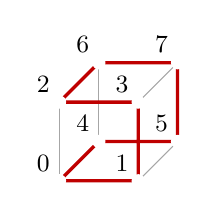
\begin{tikzpicture}[scale=1.0, every node/.style={font=\small}]
  % A simple 2D projection of the 3-cube (z=0 front square, z=1 back square offset).
  \coordinate (v0) at (0,0);
  \coordinate (v1) at (1,0);
  \coordinate (v2) at (0,1);
  \coordinate (v3) at (1,1);
  \coordinate (v4) at (0.5,0.5);
  \coordinate (v5) at (1.5,0.5);
  \coordinate (v6) at (0.5,1.5);
  \coordinate (v7) at (1.5,1.5);

  % Cube edges
  \draw[gray!70] (v0)--(v1)--(v3)--(v2)--cycle;
  \draw[gray!70] (v4)--(v5)--(v7)--(v6)--cycle;
  \draw[gray!70] (v0)--(v4) (v1)--(v5) (v2)--(v6) (v3)--(v7);

  % Gray-8 cycle path: [0,1,3,2,6,7,5,4] (and back to 0)
  \draw[red!75!black, very thick] (v0)--(v1)--(v3)--(v2)--(v6)--(v7)--(v5)--(v4)--(v0);

  % Vertex labels
  \foreach \k/\p in {0/v0,1/v1,2/v2,3/v3,4/v4,5/v5,6/v6,7/v7} {
    \filldraw[white] (\p) circle (2.2pt);
    \node[above left] at (\p) {\(\k\)};
  }
\end{tikzpicture}
\caption{A 2D projection of the 3-cube with the Gray-8 cycle highlighted:
\([0,1,3,2,6,7,5,4]\). Each step flips exactly one bit, representing an 8-tick atomic closure schedule.}
\label{fig:gray8}
\end{figure}

\paragraph{Connection to the ``$-8$'' reference.}
Later, when we define the mass law at the anchor, the appearance of a universal ``$-8$'' in the ladder exponent will be interpreted as a
coordinate origin tied to this eight-tick closure clock, not as a fitted, particle-by-particle correction. \HYP

\paragraph{Classical correspondence.}
The eight-tick minimal period ($2^D$ with $D=3$) has no direct classical analog: in continuum field theory,
microscopic periodicity is hidden beneath coarse-grained dynamics.
The closest conceptual relative is the minimal cell traversal in discrete dynamical systems,
where a state space of $2^D$ vertices requires at least $2^D$ steps for a Hamiltonian path.
In signal processing, the Nyquist--Shannon sampling theorem provides a related bound:
faithful reconstruction of a band-limited signal requires at least two samples per period.
Here the 8-tick cycle plays an analogous role as the minimal closure period for a 3-bit context. \HYP

\section{The \texorpdfstring{$\phig$}{phi}-Ladder: Self-Similarity and Scale Coordinates}
\subsection{Why a multiplicative ladder is the natural coordinate for mass hierarchies}
Particle masses span many orders of magnitude.
In such a setting, differences are less informative than \emph{ratios}: a model that treats ``one step'' as a fixed multiplicative change is more stable than a model
that treats ``one step'' as a fixed additive change.
This motivates using a logarithmic coordinate for scale.

\subsection{A self-similarity constraint that singles out \texorpdfstring{$\phig$}{phi}}
To choose a canonical base for the ladder, we impose a simple self-similarity requirement: the growth factor should be compatible with a two-step recurrence in which
the next scale decomposes into the sum of the previous two scales. \HYP
At the level of a unitless scaling factor $x$, this is captured by
\begin{equation}
  x^2 = x + 1. \HYP
  \label{eq:phi_quadratic}
\end{equation}
Equation~\eqref{eq:phi_quadratic} has a unique positive solution:
\begin{equation}
  \phig := \frac{1+\sqrt5}{2}. \PROVED
  \label{eq:phi_def}
\end{equation}
We use this $\phig$ as the base of the ladder coordinate. \HYP
The mathematical content is unambiguous (the solution exists and is unique); the modeling content is the claim that the relevant closure/self-similarity constraint
for stable recognition boundaries is correctly represented by~\eqref{eq:phi_quadratic}.

\subsection{Scale coordinates in base \texorpdfstring{$\phig$}{phi}}
Define the base-$\phig$ logarithm as
\begin{equation}
  \log_{\phig}(x) := \frac{\ln x}{\ln \phig}. \PROVED
  \label{eq:logphi_def}
\end{equation}
This coordinate has the standard ratio property:
\begin{equation}
  \log_{\phig}(m_1) - \log_{\phig}(m_2) = \log_{\phig}\!\left(\frac{m_1}{m_2}\right). \PROVED
  \label{eq:logphi_ratio}
\end{equation}

\subsection{Rungs, step size, and what ``integer'' means in this paper}
We will describe masses by integer \emph{rungs} on the $\phig$-ladder at a single anchor scale $\muStar$.
Concretely, ``rung differences'' are modeled as integer differences in the scale coordinate. \HYP
Under this convention, if two species differ by an integer rung offset $\Delta r$, their ratio at the anchor is a pure $\phig$-power:
\begin{equation}
  \frac{m_1}{m_2} = \phig^{\Delta r}. \PROVED
  \label{eq:pure_phi_ratio}
\end{equation}

\paragraph{Connection to the mass formula.}
Later, the full anchor law will introduce additional structure beyond the rung skeleton (a shared charge-derived band coordinate and sector-global yardsticks).
The role of this section is only to justify \emph{why} a $\phig$-based rung coordinate is a natural way to encode multiplicative hierarchies without per-species tuning.

\paragraph{Classical correspondence.}
The cost functional underlying the $\phig$-ladder corresponds via the Euler--Lagrange
equivalence to stationary-action principles and Dirichlet energy minimization in classical field theory.
Specifically, the symmetric cost $J(x)=\tfrac12(x+1/x)-1$ satisfies the same variational
structure as the Lagrangian density for a free scalar field in the local quadratic regime.
The golden ratio $\phig$ then emerges as the unique positive fixed point of the
self-similarity constraint $x^2=x+1$, which corresponds to the fixed-point structure
of renormalization-group flows: exponents that recur across energy scales without
requiring per-scale tuning. \HYP

\section{Sector Yardsticks from Cube Geometry}
\subsection{The counting layer: cube combinatorics and a symmetry constant}
The yardsticks used in the mass framework are \emph{sector-global}: each sector (charged leptons, up-type quarks, down-type quarks, electroweak)
shares a single baseline scale at the anchor, rather than having per-particle offsets. \PROVED

The inputs to the yardstick construction are simple integers.
First, the 3-cube has:
\[
\text{vertices}=8,\qquad \text{edges}=12,\qquad \text{faces}=6. \PROVED
\]
Second, we use the crystallographic classification constant:
\[
W := 17, \PROVED
\]
the number of plane wallpaper groups.

\paragraph{Active vs.\ passive edges (model convention).}
We will frequently refer to a split between one distinguished ``active'' edge per tick and the remaining ``passive'' edges. \HYP
Under this convention,
\[
E_{\mathrm{total}} := 12,\qquad
A_z := 1,\qquad
E_{\mathrm{passive}} := E_{\mathrm{total}} - A_z = 11. \HYP
\]
The arithmetic is trivial; the modeling content is that this particular split is the correct bookkeeping for an atomic closure clock. \HYP

\subsection{Yardstick form and what is being derived}
For each sector we use a yardstick of the form
\begin{equation}
  A_{\mathrm{sector}}
  \;:=\;
  2^{B_{\mathrm{pow}}(\mathrm{sector})}\,\Ecoh\,\phig^{r_0(\mathrm{sector})}.
  \HYP
  \label{eq:yardstick_form}
\end{equation}
Here:
\begin{itemize}
  \item \(B_{\mathrm{pow}}(\mathrm{sector})\in\mathbb Z\) is a binary gauge exponent, \HYP
  \item \(r_0(\mathrm{sector})\in\mathbb Z\) is a $\phig$-origin exponent, \HYP
  \item \(\Ecoh\) is a common coherence unit shared across sectors (defined later, with explicit unit conventions when comparing to PDG). \CERT
\end{itemize}

\paragraph{Key point (no per-flavor tuning).}
The model does \emph{not} permit choosing \(B_{\mathrm{pow}}\) or \(r_0\) separately for each particle.
Instead, the sector exponents are fixed once and for all from the counting layer. \PROVED

\subsection{Sector exponent formulas (closed form; no fitting)}
Given the counting-layer integers \((E_{\mathrm{total}},E_{\mathrm{passive}},W,A_z)\), the sector exponents are fixed by:
\begin{align}
  B_{\mathrm{pow}}(\mathrm{Lepton}) &:= -2E_{\mathrm{passive}}, &
  r_0(\mathrm{Lepton}) &:= 4W - 6, \PROVED \label{eq:lepton_yardstick_exponents}\\
  B_{\mathrm{pow}}(\mathrm{UpQuark}) &:= -A_z, &
  r_0(\mathrm{UpQuark}) &:= 2W + A_z, \PROVED \label{eq:up_yardstick_exponents}\\
  B_{\mathrm{pow}}(\mathrm{DownQuark}) &:= 2E_{\mathrm{total}} - 1, &
  r_0(\mathrm{DownQuark}) &:= E_{\mathrm{total}} - W, \PROVED \label{eq:down_yardstick_exponents}\\
  B_{\mathrm{pow}}(\mathrm{Electroweak}) &:= A_z, &
  r_0(\mathrm{Electroweak}) &:= 3W + 4. \PROVED \label{eq:ew_yardstick_exponents}
\end{align}
Substituting \(E_{\mathrm{total}}=12\), \(E_{\mathrm{passive}}=11\), \(W=17\), and \(A_z=1\) gives the sector-wide constants:
\begin{center}
\begin{tabular}{lrr}
\toprule
Sector & \(B_{\mathrm{pow}}\) & \(r_0\) \\
\midrule
Lepton & \(-22\) & \(62\) \\
Up quark & \(-1\) & \(35\) \\
Down quark & \(23\) & \(-5\) \\
Electroweak & \(1\) & \(55\) \\
\bottomrule
\end{tabular}
\end{center}
These are sector constants: they are shared across all particles in the sector and are not adjusted per species. \PROVED

\begin{figure}[t]
\centering
\begin{tikzpicture}[
  every node/.style={font=\small},
  box/.style={draw, rounded corners, align=center, inner sep=4pt},
  >=Stealth
]
  \node[box] (inputs) {Counting layer\\[2pt]
    \(E_{\mathrm{total}}=12\)\\
    \(E_{\mathrm{passive}}=11\)\\
    \(W=17\)\\
    \(A_z=1\)};

  \node[box, right=18mm of inputs, yshift=14mm] (up) {Up sector\\[2pt]
    \(B_{\mathrm{pow}}=-A_z\)\\
    \(r_0=2W+A_z\)};

  \node[box, right=18mm of inputs, yshift=-14mm] (down) {Down sector\\[2pt]
    \(B_{\mathrm{pow}}=2E_{\mathrm{total}}-1\)\\
    \(r_0=E_{\mathrm{total}}-W\)};

  \node[box, right=18mm of inputs] (lepton) {Lepton sector\\[2pt]
    \(B_{\mathrm{pow}}=-2E_{\mathrm{passive}}\)\\
    \(r_0=4W-6\)};

  \node[box, below=10mm of lepton] (ew) {EW sector\\[2pt]
    \(B_{\mathrm{pow}}=A_z\)\\
    \(r_0=3W+4\)};

  \draw[->] (inputs) -- (up);
  \draw[->] (inputs) -- (down);
  \draw[->] (inputs) -- (lepton);
  \draw[->] (inputs) -- (ew);
\end{tikzpicture}
\caption{Sector yardstick exponents are fixed from the counting layer (no per-species tuning). The only shared non-integer in the yardstick is the ladder base \(\phig\) and the coherence unit \(\Ecoh\).}
\label{fig:yardsticks}
\end{figure}

\paragraph{Interpretation.}
The role of this section is to make parameter accounting explicit:
once the counting layer and the sector map are fixed, the sector baselines are fixed.
Any remaining structure in the spectrum must come from discrete coordinates shared across families (rungs and band labels), not from hidden per-particle knobs. \PROVED

\paragraph{Classical correspondence.}
The sector yardsticks correspond to the discrete integer inputs that appear in Standard-Model
renormalization-group bookkeeping (loop counts, threshold matchings, group-theory factors).
In the SM, such integers arise from representation theory and are not fitted; here they arise from
cube combinatorics and the crystallographic constant $W=17$.
The use of dimensionless ratios to eliminate arbitrary scale choices corresponds to the
Buckingham $\Pi$-theorem of dimensional analysis: physical predictions must be expressible as
functions of dimensionless combinations of the inputs.
The sector exponents $(B_{\mathrm{pow}}, r_0)$ are the discrete analogs of anomalous dimensions
in that they determine how each sector's baseline scales under the ladder coordinate. \HYP

\section{The Single-Anchor Mass Law}
\noindent\fbox{\parbox{0.97\linewidth}{%
\textbf{Section summary.}
At a single common anchor scale \(\muStar\), the framework assigns each charged fermion a sector yardstick, an integer rung, and a charge-derived band label.
These ingredients determine an anchor mass display law.
This section states the law, defines the charge-to-band map and the closed-form band function, and records the key corollary:
within an equal-\(Z\) family, anchor mass ratios are pure \(\phig\)-powers of rung differences.}}

\subsection{Single anchor scale (what is meant by ``at \texorpdfstring{$\muStar$}{mu*}'')}
The mass law in this paper is stated at one common reference scale \(\muStar\). \HYP
Numerical comparisons to external conventions (PDG pole masses, running \(\overline{\mathrm{MS}}\) masses, etc.) are carried out only after an explicit
transport step is declared (see Sec.~7). \CERT

For concreteness we take
\[
\muStar = 182.201~\mathrm{GeV}. \CERT
\]
The value above is a declared anchor used for the paper’s reproducible tables; the physical point is that \emph{one} common anchor is used for all species,
not a different tuned anchor per particle. \PROVED

\subsection{Charge integerization and the band integer \texorpdfstring{$Z$}{Z}}
Let \(Q\) denote the electric charge in units of \(e\), and define the integerized charge
\begin{equation}
  \tildeQ := 6Q \in \mathbb Z. \HYP
  \label{eq:charge_integerization}
\end{equation}
We then define a charge-derived band integer \(Z\) by the sector-dependent rule
\begin{equation}
  \Zidx(Q,\mathrm{sector}) :=
  \begin{cases}
    \tildeQ^2 + \tildeQ^4, & \mathrm{sector}=\mathrm{lepton},\\
    4 + \tildeQ^2 + \tildeQ^4, & \mathrm{sector}=\mathrm{quark}.
  \end{cases}
  \HYP
  \label{eq:Zmap}
\end{equation}
This rule assigns a common \(Z\) value to each charged family. In particular, for the Standard Model charges
\(\tildeQ=-6\) (leptons), \(\tildeQ=4\) (up-type quarks), and \(\tildeQ=-2\) (down-type quarks), one obtains:
\begin{equation}
  Z_{\ell}=1332,\qquad Z_{u}=276,\qquad Z_{d}=24. \PROVED
  \label{eq:Z_family_values}
\end{equation}

\subsection{Closed-form band function \texorpdfstring{$\mathrm{gap}(Z)$}{gap(Z)}}
Given \(Z\), define the band function
\begin{equation}
  \mathrm{gap}(Z) := \log_{\phig}\!\left(1+\frac{Z}{\phig}\right). \HYP
  \label{eq:gap_def}
\end{equation}
This is a closed-form mapping from the charge-derived integer \(Z\) to a ladder exponent shift.
It is shared across all members of an equal-\(Z\) family. \PROVED

\subsection{The anchor display law}
Let \(A_{\mathrm{sector}}\) be the sector yardstick defined in Sec.~4, and let \(r_i\in\mathbb Z\) be an integer rung assigned to species \(i\). \HYP
The single-anchor mass law is:
\begin{equation}
  \mRS(i;\muStar)
  \;:=\;
  A_{\mathrm{sector}(i)}\,\phig^{\,r_i - 8 + \mathrm{gap}(\Zidx_i)}.
  \HYP
  \label{eq:masslaw_anchor}
\end{equation}
The universal ``\(-8\)'' is an octave reference shift (Sec.~2): a coordinate origin tied to one complete eight-tick closure, not a per-particle fit parameter. \HYP

\paragraph{Scope honesty about rungs.}
In this paper, \(r_i\) is treated as a discrete ladder coordinate.
The claim being tested in the Tier-A display is not ``we can fit every mass by choosing \(r_i\)''; instead, the test is whether a \emph{single} shared charge-to-band
rule~\eqref{eq:Zmap} and shared band function~\eqref{eq:gap_def} organize the spectrum into equal-\(Z\) families at the anchor. \HYP

\subsection{Skeleton \texorpdfstring{$\times$}{x} band: a useful factorization}
Define the rung-and-yardstick skeleton mass at the anchor by
\begin{equation}
  m_{\mathrm{skel}}(i;\muStar) := A_{\mathrm{sector}(i)}\,\phig^{\,r_i-8}. \PROVED
  \label{eq:skeleton_mass}
\end{equation}
Then the anchor law factors as
\begin{equation}
  \mRS(i;\muStar) = m_{\mathrm{skel}}(i;\muStar)\,\phig^{\mathrm{gap}(\Zidx_i)}. \PROVED
  \label{eq:masslaw_factorization}
\end{equation}
This factorization is operationally important: it separates the integer rung skeleton from the shared family band coordinate.

\subsection{Equal-\texorpdfstring{$Z$}{Z} corollary: within-family ratios are pure \texorpdfstring{$\phig$}{phi}-powers}
If two species \(i,j\) are in the same sector and share the same band label \(\Zidx_i=\Zidx_j\), then the band factor cancels in the ratio, giving
\begin{equation}
  \frac{\mRS(i;\muStar)}{\mRS(j;\muStar)} = \phig^{\,r_i-r_j}. \PROVED
  \label{eq:equalZ_ratio}
\end{equation}
Thus, within an equal-\(Z\) family, the anchor ratios are determined entirely by integer rung differences.
This is the sense in which the anchor law enforces strong structure without per-species offsets. \PROVED

\paragraph{Classical correspondence.}
The single-anchor mass law corresponds to the quantum ladder structure familiar from
atomic and nuclear physics, where discrete energy levels are indexed by integer quantum numbers.
In the SM, mass ratios within a family (e.g., $m_\tau/m_\mu$, $m_b/m_s$) are empirical inputs;
here they are constrained by integer rung differences at the anchor.
The band function $\mathrm{gap}(Z) = \log_\phig(1+Z/\phig)$ is analogous to a geometric
``residue'' that captures the family-level correction beyond the skeleton.
The equal-$Z$ corollary---that within-family ratios are pure $\phig$-powers---corresponds
to the cancellation of common scale factors in dimensionless observables, a standard
feature of renormalization-group analyses where absolute scales cancel from ratios. \HYP

\section{Lepton Mass Chain (T9/T10)}
\noindent\fbox{\parbox{0.97\linewidth}{%
\textbf{Section summary.}
The anchor law of Sec.~5 organizes the charged spectrum at \(\muStar\).
This section presents an additional, lepton-specific pipeline that yields absolute predictions for
\(m_e\), \(m_\mu\), and \(m_\tau\) as a sequence of derived ladder exponents.
The pipeline has two parts: (i) an electron ``break'' exponent (a large shift) fixed from the same counting layer and coupling constant \(\alpha\),
and (ii) generation-step exponents from electron\(\to\)muon and muon\(\to\)tau.
All numerical comparisons are labeled as validation against PDG.}}

\subsection{Electron baseline at the anchor}
For leptons the family band label is \(Z_\ell=1332\) (Sec.~5). \PROVED
Write the lepton skeleton mass at the anchor as
\begin{equation}
  m_{\mathrm{skel}}(e;\muStar) := A_{\mathrm{Lepton}}\,\phig^{\,r_e-8}. \PROVED
  \label{eq:electron_skeleton}
\end{equation}
Then the anchor display law specializes to
\begin{equation}
  \mRS(e;\muStar) = m_{\mathrm{skel}}(e;\muStar)\,\phig^{\mathrm{gap}(1332)}. \PROVED
  \label{eq:electron_anchor_display}
\end{equation}
This anchor display is an organizational coordinate statement; by itself it is not yet the low-energy electron mass. \HYP

\subsection{The electron break (refined shift)}
To obtain an absolute electron mass prediction, we introduce a lepton-specific exponent shift \(\delta_e\) (the ``break''). \HYP
It is fixed by the same integer layer \((W,E_{\mathrm{total}},E_{\mathrm{passive}})\) together with the fine-structure constant \(\alpha\): \HYP
\begin{equation}
  \delta_e
  \;:=\;
  2W \;+\; \frac{W + E_{\mathrm{total}}}{4E_{\mathrm{passive}}}
  \;+\; \alpha^2 \;+\; E_{\mathrm{total}}\alpha^3.
  \HYP
  \label{eq:delta_e}
\end{equation}
The interpretation is that the first two terms capture a purely topological ledger contribution, while the latter two terms are small radiative corrections
organized by \(\alpha\). \HYP

With \(\delta_e\) fixed, the electron mass prediction is
\begin{equation}
  m_e^{\mathrm{pred}}
  \;:=\;
  m_{\mathrm{skel}}(e;\muStar)\,\phig^{\mathrm{gap}(1332)-\delta_e}.
  \HYP
  \label{eq:me_pred}
\end{equation}

\subsection{Generation steps: \texorpdfstring{electron\(\to\)muon\(\to\)tau}{electron to muon to tau}}
The muon and tau are obtained by adding two step exponents to the electron residue. \HYP
Define the electron\(\to\)muon step as
\begin{equation}
  S_{e\to\mu}
  \;:=\;
  E_{\mathrm{passive}} \;+\; \frac{1}{4\pi} \;-\; \alpha^2.
  \HYP
  \label{eq:step_emu}
\end{equation}
The leading term \(E_{\mathrm{passive}}=11\) is an integer rung jump; the remaining terms provide small geometry/coupling corrections. \HYP

Define the muon\(\to\)tau step as
\begin{equation}
  S_{\mu\to\tau}
  \;:=\;
  6 \;-\; \frac{2W+3}{2}\,\alpha.
  \HYP
  \label{eq:step_mutau}
\end{equation}
The leading term \(6\) is again an integer jump (the cube face count), with a small \(\alpha\)-dependent correction. \HYP

Using these steps, the muon and tau predictions are
\begin{align}
  m_\mu^{\mathrm{pred}}
  &:= m_{\mathrm{skel}}(e;\muStar)\,\phig^{\mathrm{gap}(1332)-\delta_e + S_{e\to\mu}},
  \HYP
  \label{eq:mmu_pred}\\
  m_\tau^{\mathrm{pred}}
  &:= m_{\mathrm{skel}}(e;\muStar)\,\phig^{\mathrm{gap}(1332)-\delta_e + S_{e\to\mu} + S_{\mu\to\tau}}.
  \HYP
  \label{eq:mtau_pred}
\end{align}

\subsection{Validation table (PDG comparison)}
We report the numerical predictions in MeV under the declared unit convention (Sec.~4) and compare to PDG values \cite{PDG2024}. \VAL
The table below is generated automatically from the repository scripts (no manual editing). \PROVED

% Auto-generated by tools/lepton_chain_table.py
\begin{table}[h]
  \centering
  \caption{Lepton chain prediction (T9--T10) from first-principles constants. Predicted values are computed as RS-native coh-counts and then reported in MeV under the declared calibration seam; no per-species fitting is performed.}
  \label{tab:lepton_chain_pred_vs_pdg}
  \begin{tabular}{lrrrr}
    \toprule
    Species & Pred. (MeV) & PDG (MeV) & Abs. err & Rel. err \\
    \midrule
    e & 0.510999 & 0.510999 & -1.9546e-07 & -3.82506e-07 \\
    mu & 105.658 & 105.658 & -0.000112323 & -1.06307e-06 \\
    tau & 1776.71 & 1776.86 & -0.154158 & -8.67587e-05 \\
    \bottomrule
  \end{tabular}
\end{table}


\paragraph{Classical correspondence.}
The lepton mass chain has no direct classical analog in the Standard Model, where the
electron, muon, and tau masses are independent Yukawa inputs.
The closest conceptual relatives are:
(i)~topological linking arguments (Jordan curve theorem, Alexander polynomials) that assign
integer invariants to knotted configurations, analogous to how the generation steps
$S_{e\to\mu}$ and $S_{\mu\to\tau}$ are fixed by integer counts $(E_{\mathrm{passive}}, F)$; and
(ii)~radiative correction hierarchies in QED, where $\alpha$-dependent terms appear as
perturbative shifts to leading-order results.
The key difference is that the lepton chain fixes the $\alpha$-corrections from the same
integer layer rather than fitting them to data. \HYP

\section{Transport and PDG Comparison}
\noindent\fbox{\parbox{0.97\linewidth}{%
\textbf{Section summary.}
Any comparison to external mass conventions is scheme- and scale-dependent.
We therefore separate two distinct roles:
the structural band coordinate \(\mathrm{gap}(Z)\) (large, family-defining) and the Standard-Model RG transport exponent \(f^{RG}\)
(small, bookkeeping-only).
We explicitly do \emph{not} identify \(f^{RG}\) with \(\mathrm{gap}(Z)\).}}

\subsection{What a ``PDG mass'' means (why transport is unavoidable)}
The phrase ``the mass of a particle'' is not a single number in quantum field theory.
Depending on the particle and convention, quoted values may refer to:
\begin{itemize}
  \item \textbf{Pole masses} (commonly used for charged leptons), or
  \item \textbf{running masses} (commonly used for quarks in \(\overline{\mathrm{MS}}\)) evaluated at a stated scale.
\end{itemize}
Therefore, any numerical objection or comparison must state the target \((\text{scheme},\mu)\). \PROVED

\subsection{Two different exponents (do not conflate)}
The structural band coordinate is
\[
  f^{\mathrm{Rec}}(Z) := \mathrm{gap}(Z). \PROVED
\]
It is a closed-form, family-defining exponent shift (order \(\sim 6\)--\(14\) for the charged families). \PROVED

By contrast, the RG transport exponent \(f^{RG}\) is a scheme/scale bookkeeping quantity defined from the Standard Model running mass \(m_i(\mu)\) by
\begin{equation}
  \fRG_i(\mu_1,\mu_2)
  \;:=\;
  \log_{\phig}\!\left(\frac{m_i(\mu_2)}{m_i(\mu_1)}\right)
  \;=\;
  \frac{1}{\ln\phig}\ln\!\left(\frac{m_i(\mu_2)}{m_i(\mu_1)}\right).
  \CERT
  \label{eq:frg_def}
\end{equation}
In typical SM running between \(\muStar\) and low-energy reference points, \(f^{RG}\) is small (order \(10^{-2}\) to \(10^{-1}\) for leptons). \CERT
It is therefore neither conceptually nor numerically plausible to identify \(\fRG\) with \(\mathrm{gap}(Z)\). \PROVED

\subsection{Transport display (bookkeeping only)}
Given a declared target scheme/scale \(\muT\), the transport display is
\begin{equation}
  \mPred(i;\muT)
  \;:=\;
  \mRS(i;\muStar)\,\phig^{\fRG_i(\muStar,\muT)}.
  \CERT
  \label{eq:transport_display}
\end{equation}
\noindent
\textbf{Crucial distinction:} Eq.~\eqref{eq:transport_display} is bookkeeping that aligns an anchor-defined quantity with an external convention.
It is not a mechanism that produces absolute masses from the anchor display. \PROVED
For the charged leptons in this paper, the absolute predictions are provided by the separate lepton chain of Sec.~6. \PROVED

\subsection{Pinned transport policy used for reproducible tables (CERT)}
To make the bookkeeping convention auditable, the repository pins a specific transport policy (loop orders, thresholds, integrator, and targets)
and provides a reproducible certificate of the resulting transport exponents. \CERT
We include the certificate table here to emphasize the order-of-magnitude separation between transport and band structure:

% Auto-generated by tools/rg_transport_table.py
% Policy details: QCD=4L, QED=2L, $\alpha$-run=0L, RK4=10000/ln, thresholds=(1.27,4.18,162.5)\,GeV
\begin{table}[h]
  \centering
  \caption{Pinned SM RG transport exponent certificate (CERT). Policy=\texttt{RS\_CANONICAL\_2025\_Q4}, anchor $\mu_\star=182.201\,\mathrm{GeV}$. (QCD=4L, QED=2L, $\alpha$-run=0L, RK4=10000/ln, thresholds=(1.27,4.18,162.5)\,GeV). These values are used only for scheme/scale bookkeeping and must not be conflated with $\mathrm{gap}(Z)$.}
  \begin{tabular}{lrr}
    \toprule
    Species & $\mu_{\mathrm{end}}$ [GeV] & $f^{RG}(\mu_\star,\mu_{\mathrm{end}})$ \\
    \midrule
    e & 0.000510999 & 0.0494258 \\
    mu & 0.105658 & 0.0287906 \\
    tau & 1.77686 & 0.0178757 \\
    u & 2 & 0.482193 \\
    d & 2 & 0.476388 \\
    s & 2 & 0.476388 \\
    c & 1.27 & 0.547013 \\
    b & 4.18 & 0.380746 \\
    t & 162.5 & 0.00979749 \\
    \bottomrule
  \end{tabular}
\end{table}


\subsection{The diagnostic band test (how to test \texorpdfstring{$\mathrm{gap}(Z)$}{gap(Z)} against transported data)}
If one wants to test whether the charge-derived band map clusters the charged families at the anchor, the correct diagnostic is to
transport the external mass data back to the anchor under the declared RG policy:
\begin{align}
  \mdata(i;\muStar)
  &:= \mdata(i;\muT)\,\phig^{-\fRG_i(\muStar,\muT)}, \VAL \label{eq:data_to_anchor}\\
  f_i^{\mathrm{exp}}(\muStar)
  &:= \log_{\phig}\!\left(\frac{\mdata(i;\muStar)}{m_{\mathrm{skel}}(i;\muStar)}\right). \VAL \label{eq:fexp_def}
\end{align}
Then the band-map validation statement is that \(f_i^{\mathrm{exp}}(\muStar)\) clusters by equal \(Z\) and is consistent with \(\mathrm{gap}(Z_i)\)
under the declared transport policy. \VAL

\subsection{Reviewer checklist for any numerical comparison}
Any numerical objection or alternative comparison must specify:
\begin{itemize}
  \item the target scheme (pole vs.\ \(\overline{\mathrm{MS}}\) vs.\ other),
  \item the target scale \(\muT\),
  \item the RG policy choices (loop orders, thresholds, coupling treatment, integrator), and
  \item the exact statement being tested (anchor organization vs.\ absolute-mass pipeline).
\end{itemize}

\paragraph{Classical correspondence.}
The transport exponent $f^{RG}$ is mathematically identical to the standard logarithmic
running of masses under Standard-Model renormalization-group evolution.
The distinction emphasized in this section---that $f^{RG}$ is bookkeeping while
$\mathrm{gap}(Z)$ is structural---corresponds to the distinction in effective field
theory between scheme-dependent running and scheme-independent physical observables.
The transport display Eq.~\eqref{eq:transport_display} is the analog of an RG-improved
prediction: a fixed-point quantity (the anchor mass) is transported to a comparison scale
using the SM beta functions.
The key difference is that the anchor mass itself is derived from discrete structure,
not fitted to data at any scale. \CERT

\section{Ablations and Falsifiers}
\noindent\fbox{\parbox{0.97\linewidth}{%
\textbf{Section summary.}
The goal of this paper is not merely to fit numbers; it is to propose a small set of structural ingredients that can be \emph{refuted}.
We therefore list ablations (remove one ingredient and observe failure) and falsifiers (observations that would rule out the framework).
The tests below are phrased so that a skeptical reader can reproduce them with alternative scheme/scale choices, provided the choices are stated explicitly.}}

\subsection{Ablations (drop one ingredient and see what breaks)}
\paragraph{Ablation A: remove the quark offset in the \(Z\)-map.}
Replace the quark branch of Eq.~\eqref{eq:Zmap} by \(Z=\tildeQ^2+\tildeQ^4\) (i.e.\ drop the ``\(+4\)''). \HYP
Then the charged-family labeling no longer separates cleanly between up-type and down-type quarks at the anchor: the equal-\(Z\) family clustering that motivates
the band coordinate fails. \VAL

\paragraph{Ablation B: remove the quartic term in the \(Z\)-map.}
Replace Eq.~\eqref{eq:Zmap} by a purely quadratic rule (drop \(\tildeQ^4\)). \HYP
Then the three charged-family \(Z\) values cannot be realized in the required hierarchy, and the band function \(\mathrm{gap}(Z)\) no longer produces the
observed separation between the three charged families. \VAL

\paragraph{Ablation C: change charge integerization.}
Replace \(\tildeQ=6Q\) in Eq.~\eqref{eq:charge_integerization} by \(\tildeQ=kQ\) with \(k\neq 6\) (e.g.\ \(k=3\) or \(k=5\)). \HYP
Then the Standard Model charge set does not map to a stable, sector-consistent integer family labeling, and the equal-\(Z\) family structure breaks. \VAL

\paragraph{Ablation D: remove band structure (skeleton-only).}
Drop the band factor entirely by setting \(\mathrm{gap}(Z)\equiv 0\) in Eq.~\eqref{eq:masslaw_anchor}. \HYP
The remaining skeleton \(m_{\mathrm{skel}}(i;\muStar)\) cannot reproduce the observed charged spectrum without per-species tuning, which is forbidden by the model contract. \VAL

\subsection{Falsifiers (observations that would rule out the framework)}
\paragraph{Falsifier 1: failure of equal-\(Z\) clustering at the anchor.}
Using the diagnostic protocol of Sec.~7 (Eqs.~\eqref{eq:data_to_anchor}--\eqref{eq:fexp_def}) under a declared transport policy,
compute \(f_i^{\mathrm{exp}}(\muStar)\) for the charged fermions.
If the values do not cluster by the three family labels \(Z\in\{24,276,1332\}\), the charge-derived band hypothesis is refuted. \VAL

\paragraph{Falsifier 2: need for per-particle offsets.}
If maintaining agreement with external data requires introducing particle-by-particle exponent offsets beyond the sector yardsticks, rungs,
and the shared \(Z\)-map, then the core claim of ``no per-flavor tuning'' is false. \VAL

\paragraph{Falsifier 3: lepton chain failure beyond declared tolerance.}
The lepton absolute pipeline of Sec.~6 makes a concrete numerical prediction for \(m_e,m_\mu,m_\tau\) under a declared unit convention. \VAL
If future refined measurements (or corrected convention choices) move the PDG targets outside the declared tolerance band of the prediction pipeline,
then the lepton chain is refuted as a universal mechanism. \VAL

\paragraph{Falsifier 4: scheme/scale dependence masquerading as structure.}
If the qualitative conclusions of the framework (family clustering at the anchor; order-of-magnitude separation between \(\mathrm{gap}(Z)\) and \(f^{RG}\);
and the lepton-chain hierarchy) disappear under reasonable alternative scheme/scale declarations, then the framework is not describing an invariant structural signal. \VAL

\paragraph{Classical correspondence.}
The ablation and falsification methodology corresponds to standard hypothesis testing in physics:
ablations are analogous to removing terms from a Lagrangian to check which are essential,
while falsifiers are analogous to the critical tests that distinguish competing theories.
The key methodological point is that the framework is designed to be \emph{refutable}:
unlike a fit with enough free parameters to match any data, the discrete structure here
makes sharp predictions that can fail. \VAL

